\documentclass[a4paper,landscape,hidelinks,14pt]{extarticle}

\usepackage[T2A]{fontenc}
\usepackage[utf8]{inputenc}
\usepackage[russian]{babel}
\usepackage{cmap}

\usepackage{xcolor}

\usepackage{helvet}
\usepackage{pscyr}

\usepackage{multicol}

\usepackage{amssymb,amsfonts,amsmath,mathtext}
\usepackage{cite,enumerate,float}

\usepackage{listings}
\usepackage{tikz}

\graphicspath{{images/}}           % Подключаемые пакеты
../../../templates/presentation/sys/styles.tex             % Пользовательские стили

\begin{document}
../../../templates/magistracy_dissertation_synopsis/sys/names.tex              % Переопределение именований

Объект \( \eta = \alpha + \beta \xi, \alpha = 0 \),
где \( \xi \) и \( \eta \) --- фактические значения входа и выхода,
\( \alpha, \beta \) --- фактические значения параметров.

Наблюдаются вход \( x = \xi + \epsilon \), выход \( y = \eta + \delta \),
так что \( x \) и \( y \) --- наблюдения входа и выхода.
С.к.о. ошибок измерений \( \sigma_{\epsilon}, \sigma_{\delta} \).

Значения \( \xi \) выбирались из равномерного в \( [0, 10] \) распределения.
Для получения одной оценки \( ( \alpha, \beta ) \) использовались 100 наблюдений
\( ( x_i, y_i ), i = \overline{1, 100} \). Расчеты расстояний по параметрам и по выходу
велись в узлах сетки значений \( \sigma_x, \sigma_y \) в прямоугольнике
\( [0, 2] \times [0, 2] \) с шагом 0{,}1. В каждом узле сетки вычислялось 100 оценок.

На приведенных ниже графиках
\textbf{линиями равного уровня} обозначены зависимости
разности точностей оценок параметров, полученных МНК и методом Пирсона, от
с.к.о. ошибок измерений входной и выходной переменной;
\textbf{\color{red}{красными точками}} обозначены пары значений с.к.о. ошибок измерений,
при которых данные разности имеют значения, близкие к нулю (\( -0{,}05 \ldots 0{,}05 \));
\textbf{\color{red}{прямая красного цвета}} соответствует линейной функции,
аппроксимирующей данные пары значений (методом симметричной аппроксимации по Пирсону),
а \textbf{\color{blue}{прямая синего цвета}} соответствует линейной функции вида
\begin{equation}
  \label{eq:divider}
  \sigma_{\delta} = (|\beta| + 0{,}7) \sigma_{\epsilon}.
\end{equation}

Графики расположены по порядку увеличения значения коэффициента усиления \( \beta \).

Предлагаю использовать выражение \eqref{eq:divider} для принятия решения,
какой метод следует предпочесть, по следующим причинам:
\begin{itemize}
\item его значения расположены достаточно близко к линиям нулевого уровня во всех
  рассматриваемых случаях, кроме того, когда коэффициент усиления модели равен нулю
  (рисунок~\ref{fig:beta-0});
\item оно учитывает случаи, когда коэффициент усиления отрицательный
  (рисунки~\ref{fig:beta--5}--\ref{fig:beta--0,2});
\item оно имеет более простой вид, чем предложенное вами
  (\( \sigma_{\delta} = (\beta + 0{,}6) \sigma_{\epsilon} + 0{,}1 \)).
\end{itemize}

\begin{figure}[h!]
  \centering
  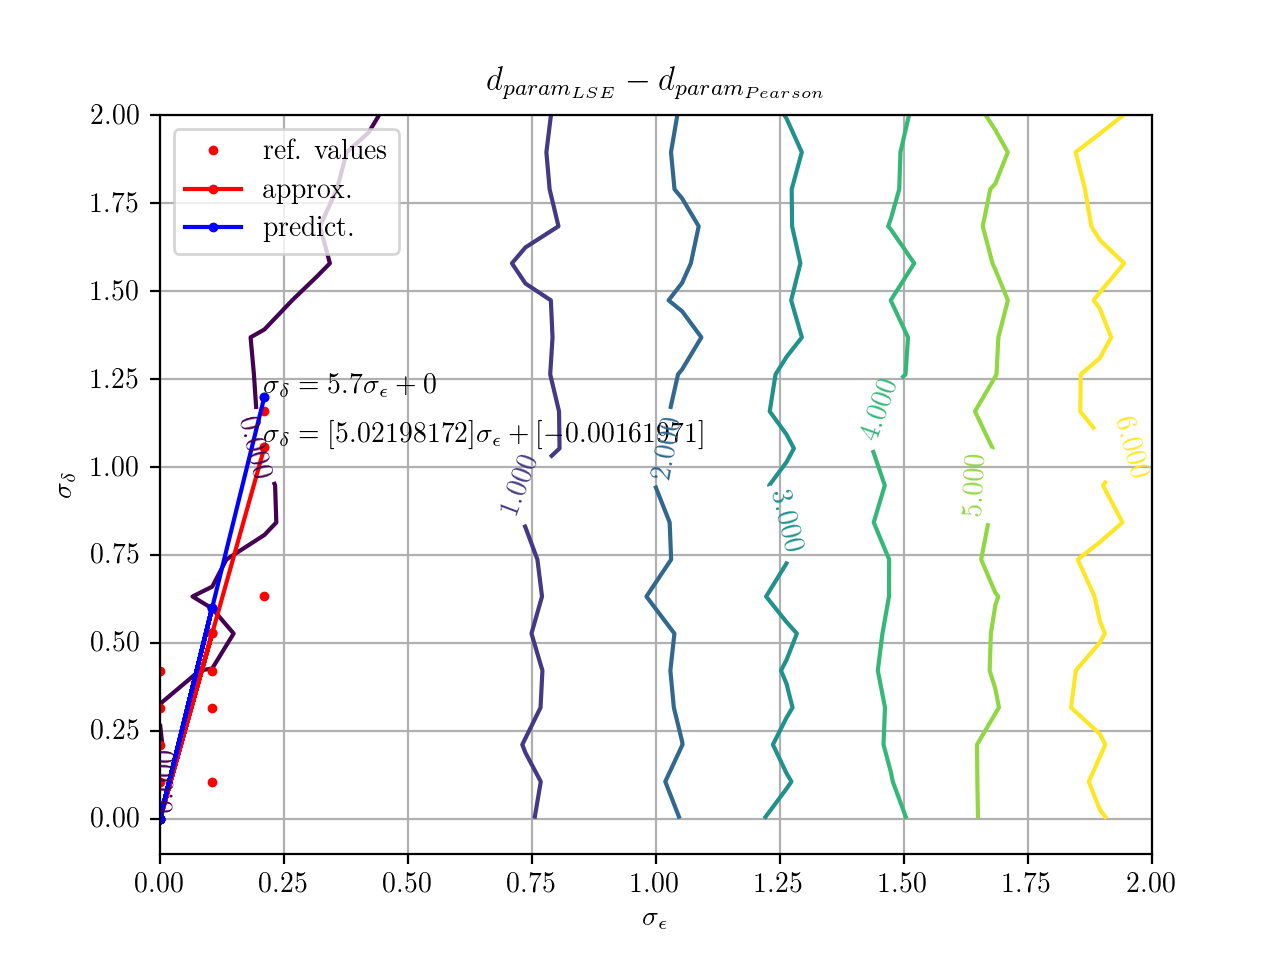
\includegraphics[width=.8\linewidth]{fig/beta--5_param-accs-diff-approx.png}
  \caption{$ \beta = -5 $}\label{fig:beta--5}
\end{figure}

\begin{figure}[h!]
  \centering
  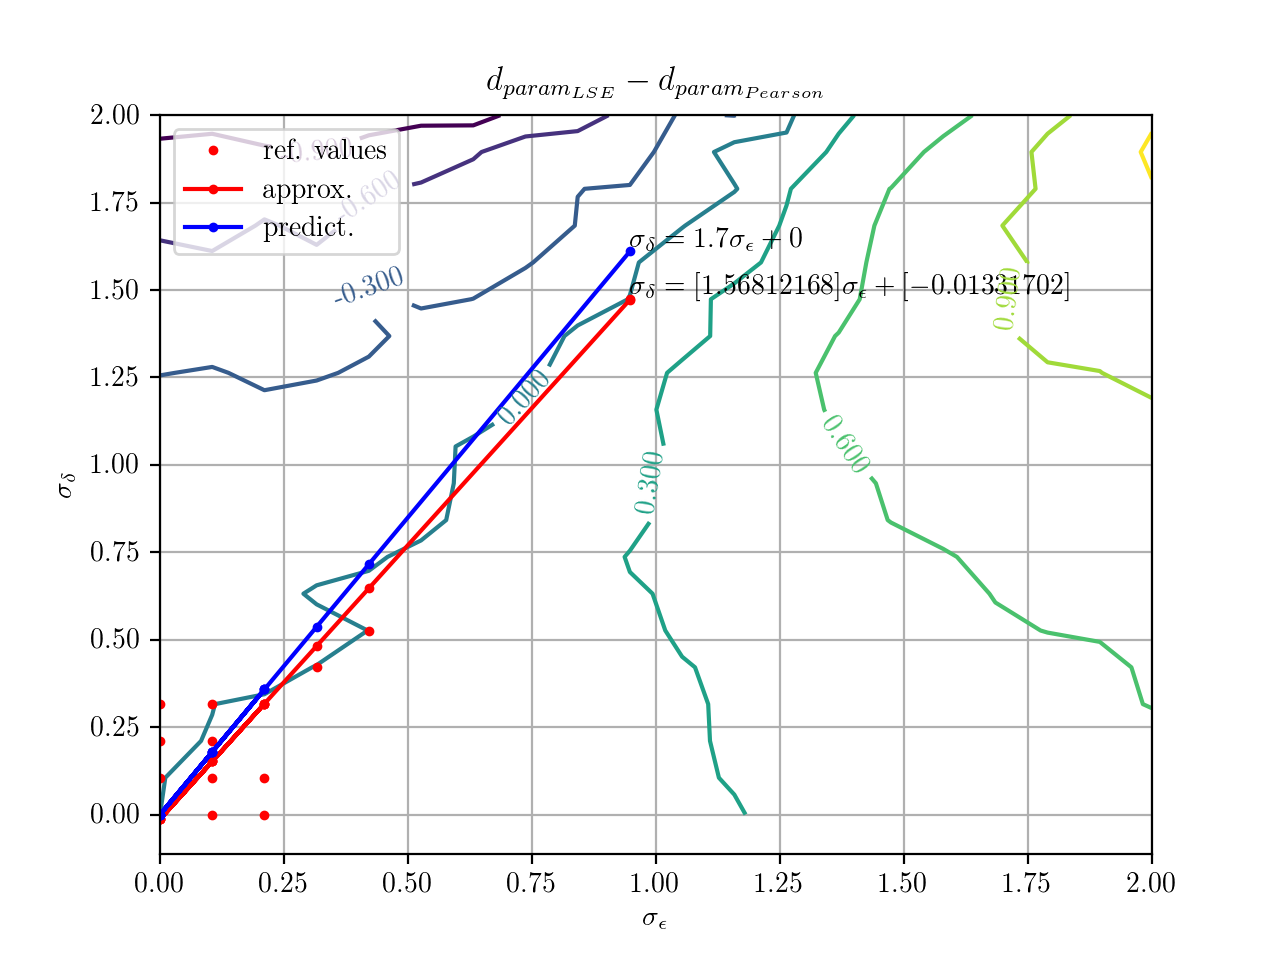
\includegraphics[width=.8\linewidth]{fig/beta--1_param-accs-diff-approx.png}
  \caption{$ \beta = -1 $}\label{fig:beta--1}
\end{figure}

\begin{figure}[h!]
  \centering
  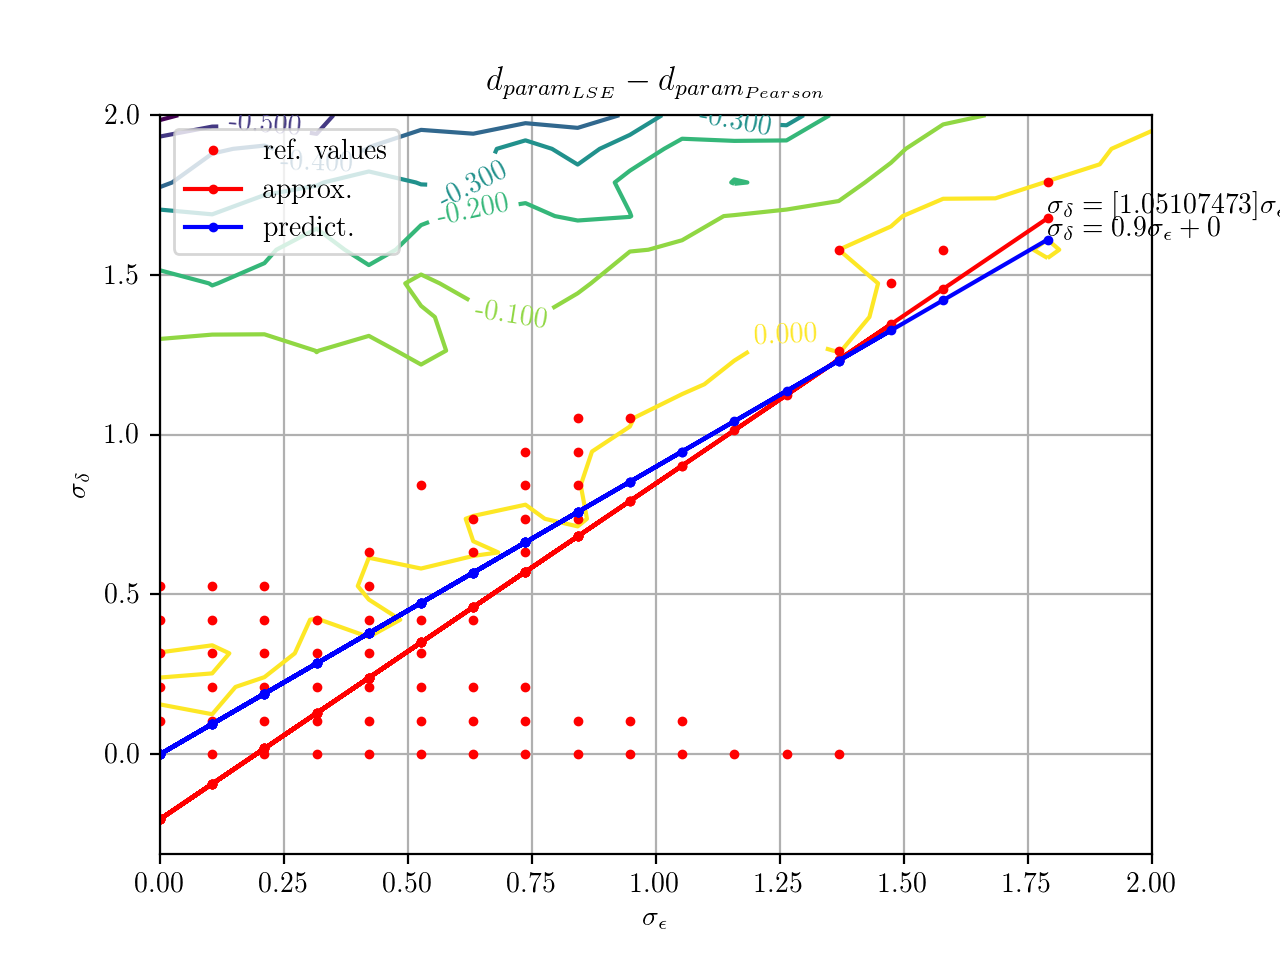
\includegraphics[width=.8\linewidth]{fig/beta--0,2_param-accs-diff-approx.png}
  \caption{$ \beta = -0{,}2 $}\label{fig:beta--0,2}
\end{figure}

\begin{figure}[h!]
  \centering
  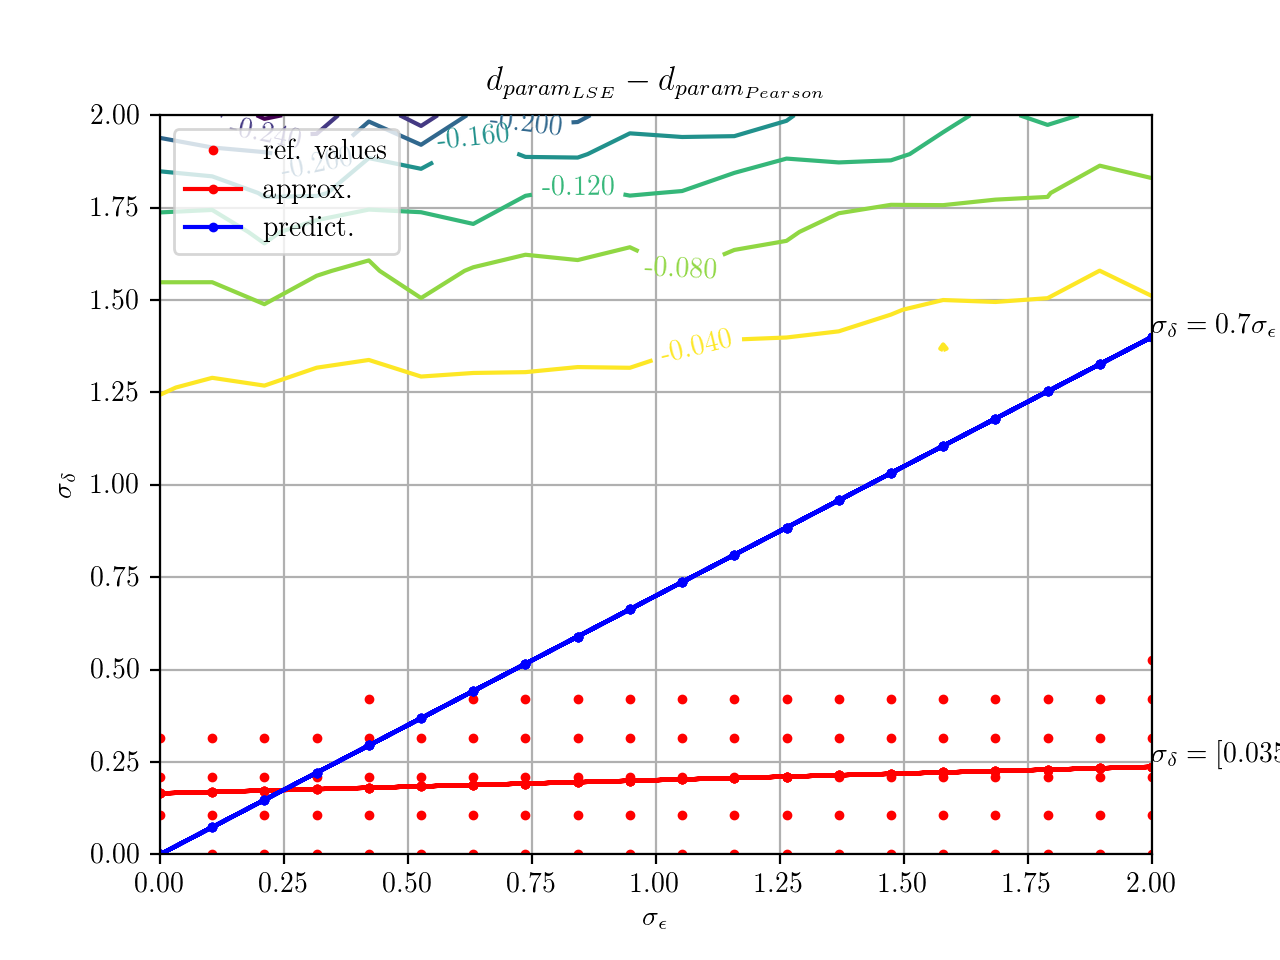
\includegraphics[width=.8\linewidth]{fig/beta-0_param-accs-diff-approx.png}
  \caption{$ \beta = 0 $}\label{fig:beta-0}
\end{figure}

\begin{figure}[h!]
  \centering
  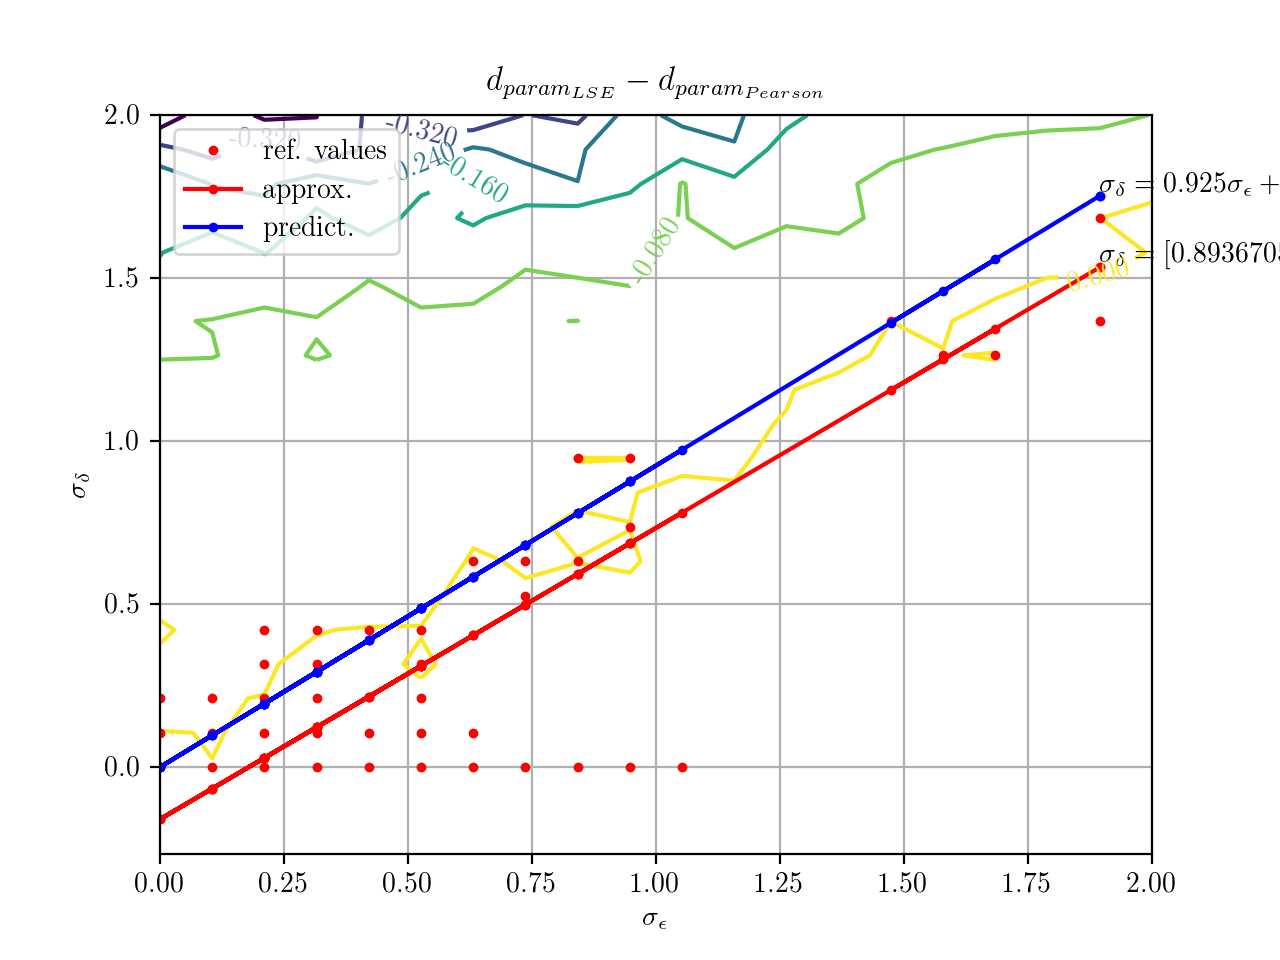
\includegraphics[width=.8\linewidth]{fig/beta-0,125_param-accs-diff-approx.png}
  \caption{$ \beta = 0{,}125 $}
\end{figure}

\begin{figure}[h!]
  \centering
  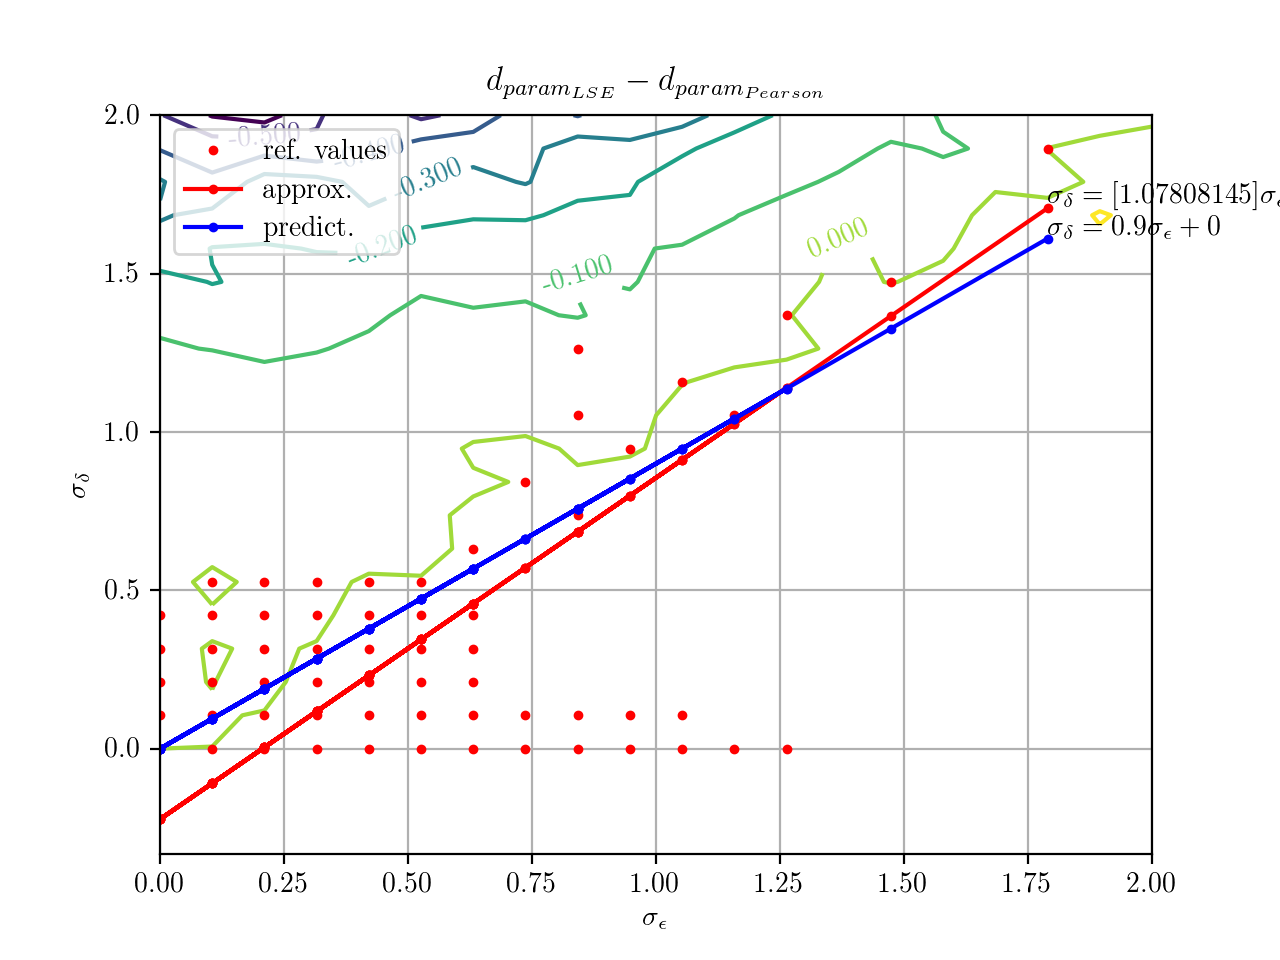
\includegraphics[width=.8\linewidth]{fig/beta-0,2_param-accs-diff-approx.png}
  \caption{$ \beta = 0{,}2 $}
\end{figure}

\begin{figure}[h!]
  \centering
  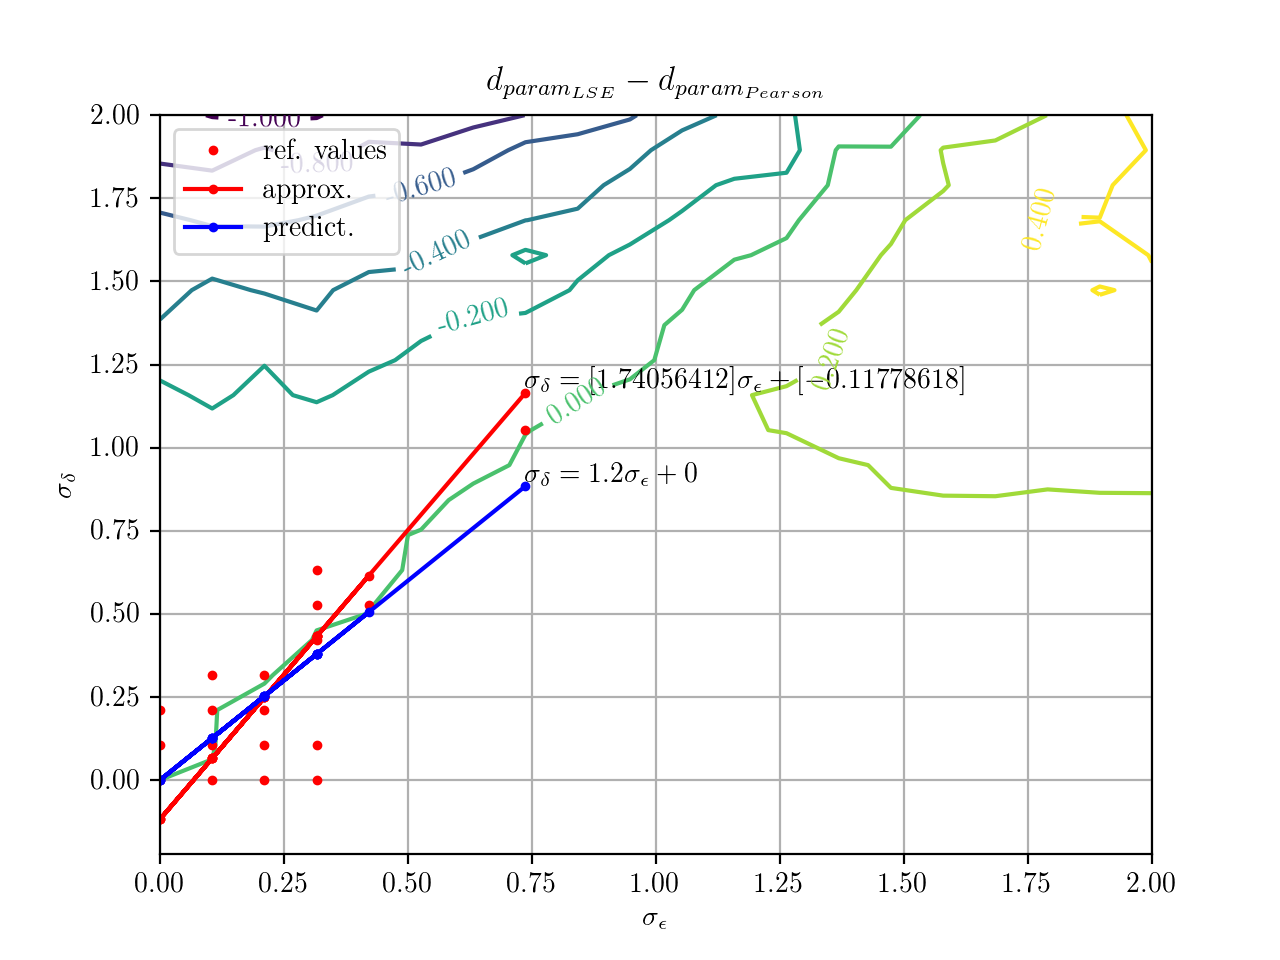
\includegraphics[width=.8\linewidth]{fig/beta-0,5_param-accs-diff-approx.png}
  \caption{$ \beta = 0{,}5 $}
\end{figure}

\begin{figure}[h!]
  \centering
  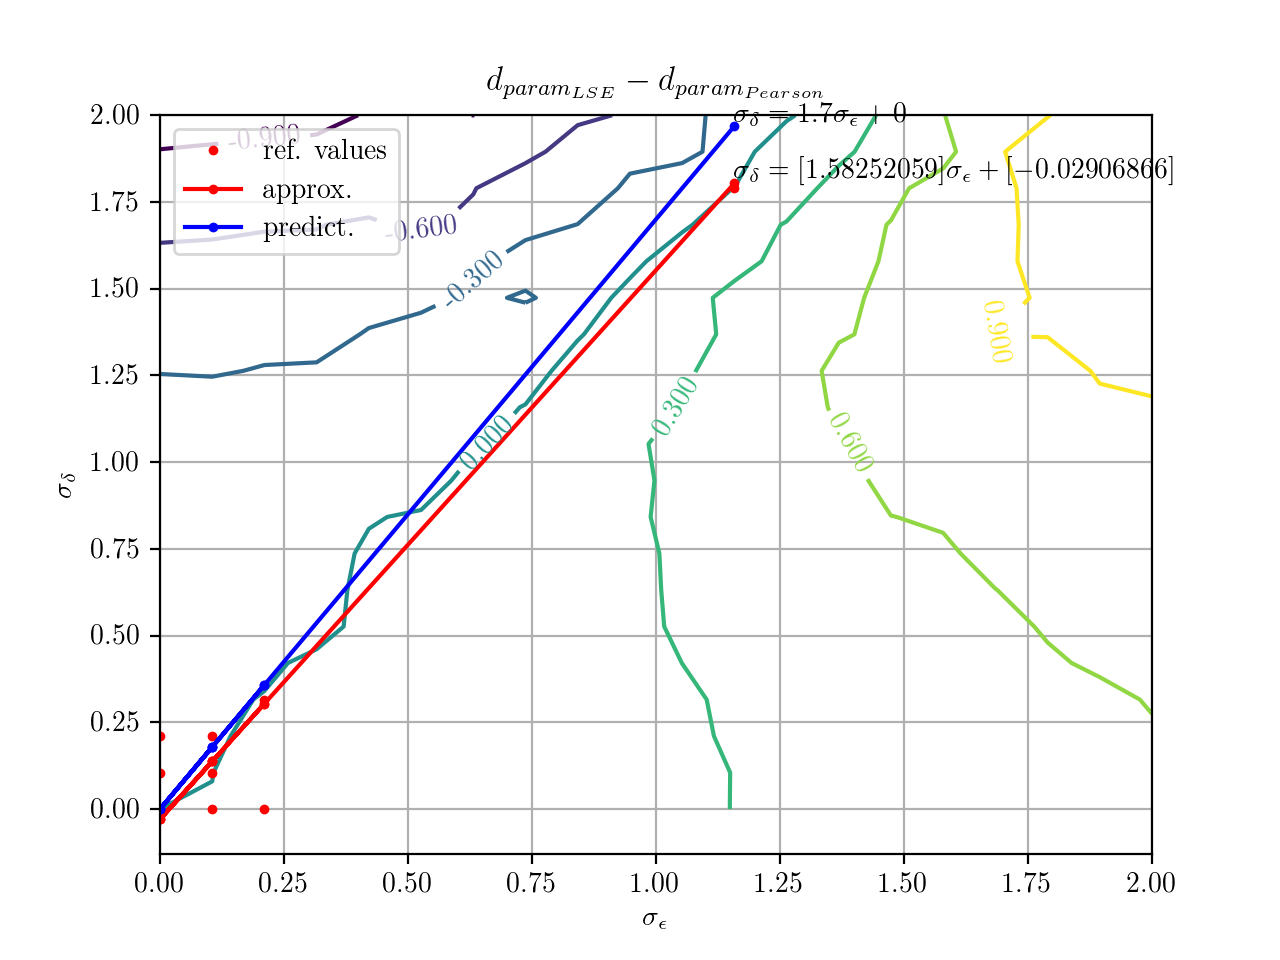
\includegraphics[width=.8\linewidth]{fig/beta-1_param-accs-diff-approx.png}
  \caption{$ \beta = 1 $}
\end{figure}

\begin{figure}[h!]
  \centering
  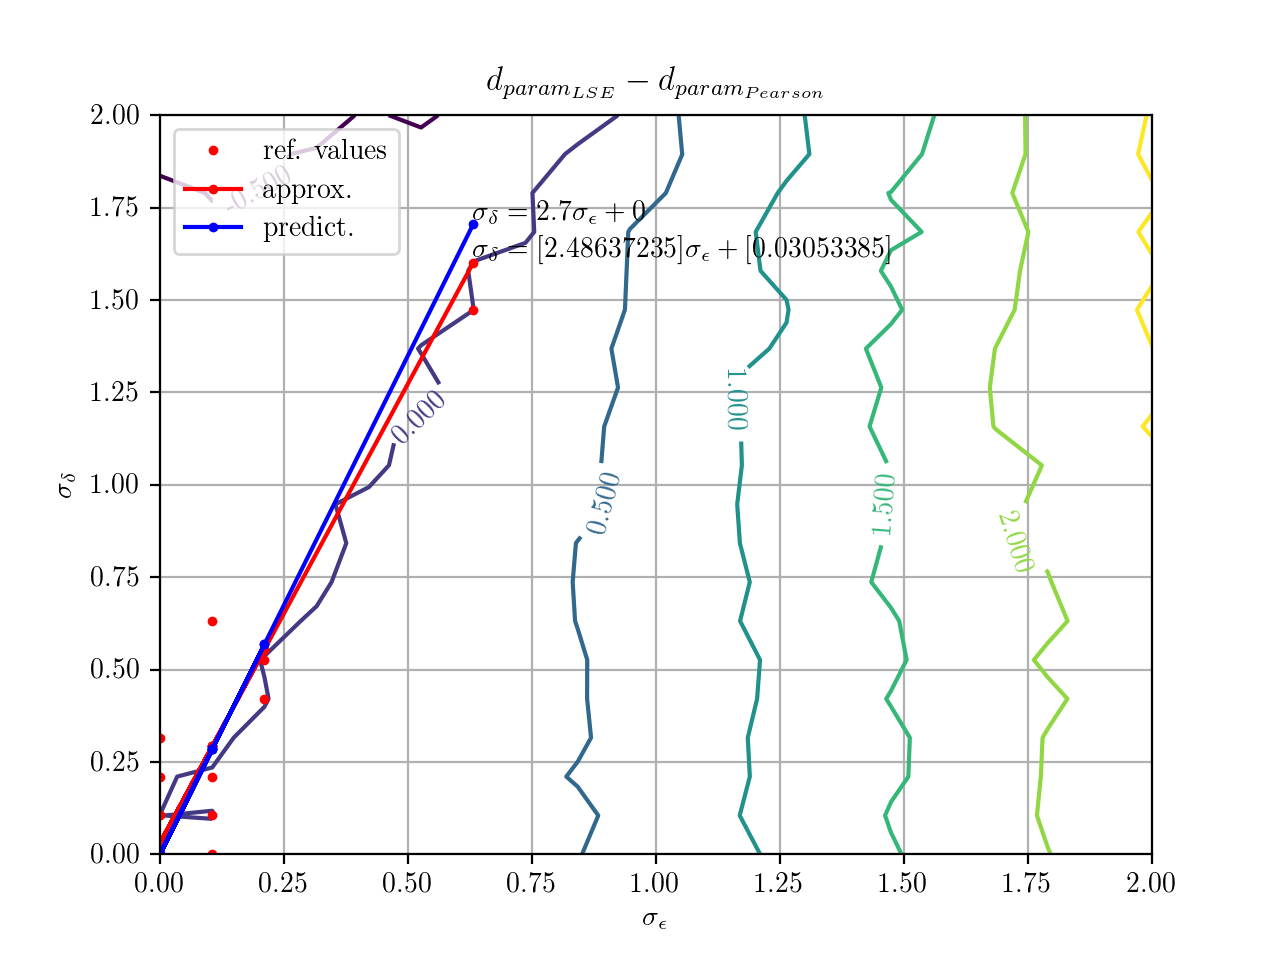
\includegraphics[width=.8\linewidth]{fig/beta-2_param-accs-diff-approx.png}
  \caption{$ \beta = 2 $}
\end{figure}

\begin{figure}[h!]
  \centering
  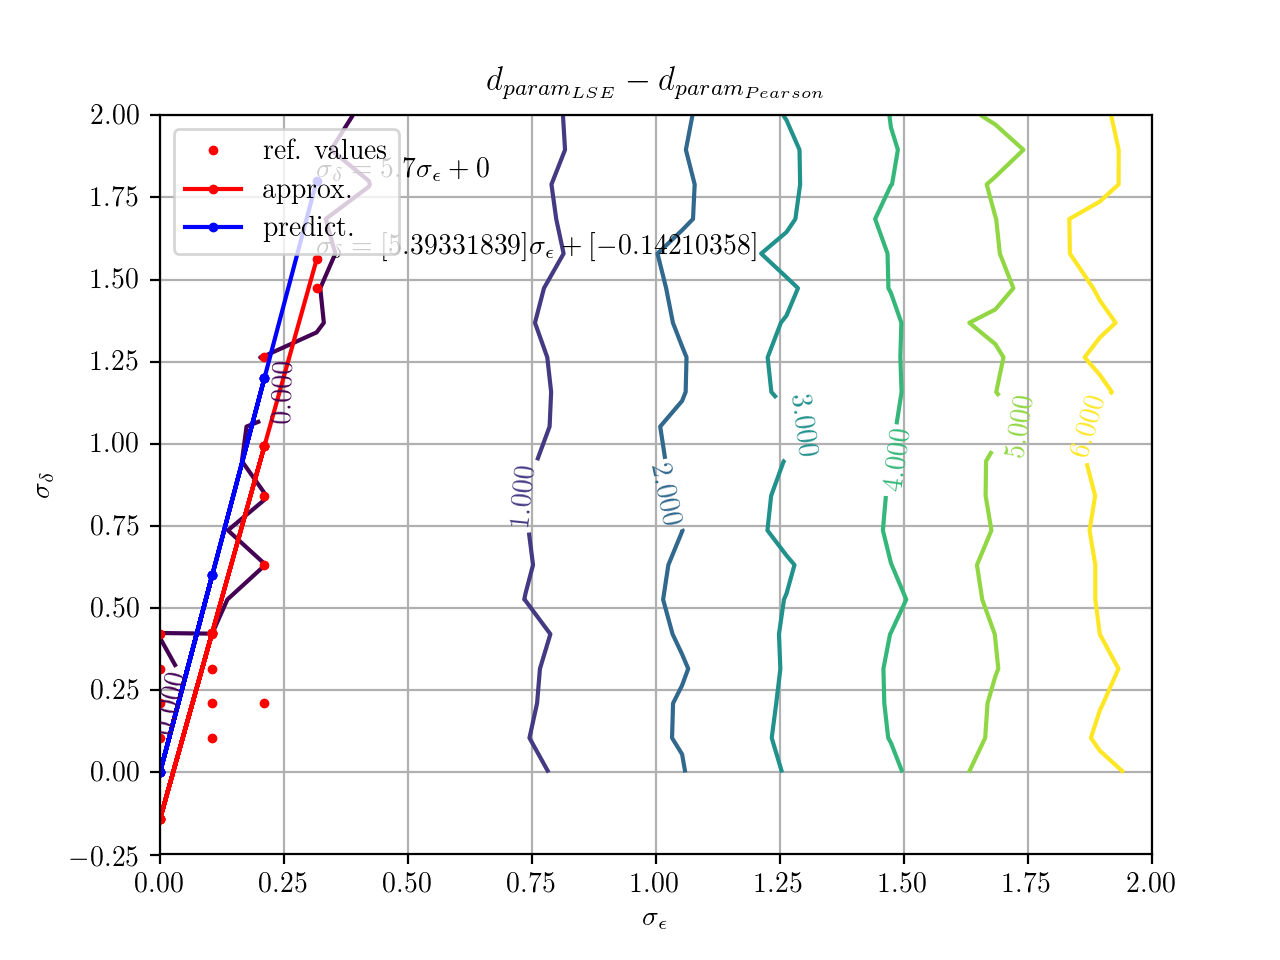
\includegraphics[width=.8\linewidth]{fig/beta-5_param-accs-diff-approx.png}
  \caption{$ \beta = 5 $}
\end{figure}

\begin{figure}[h!]
  \centering
  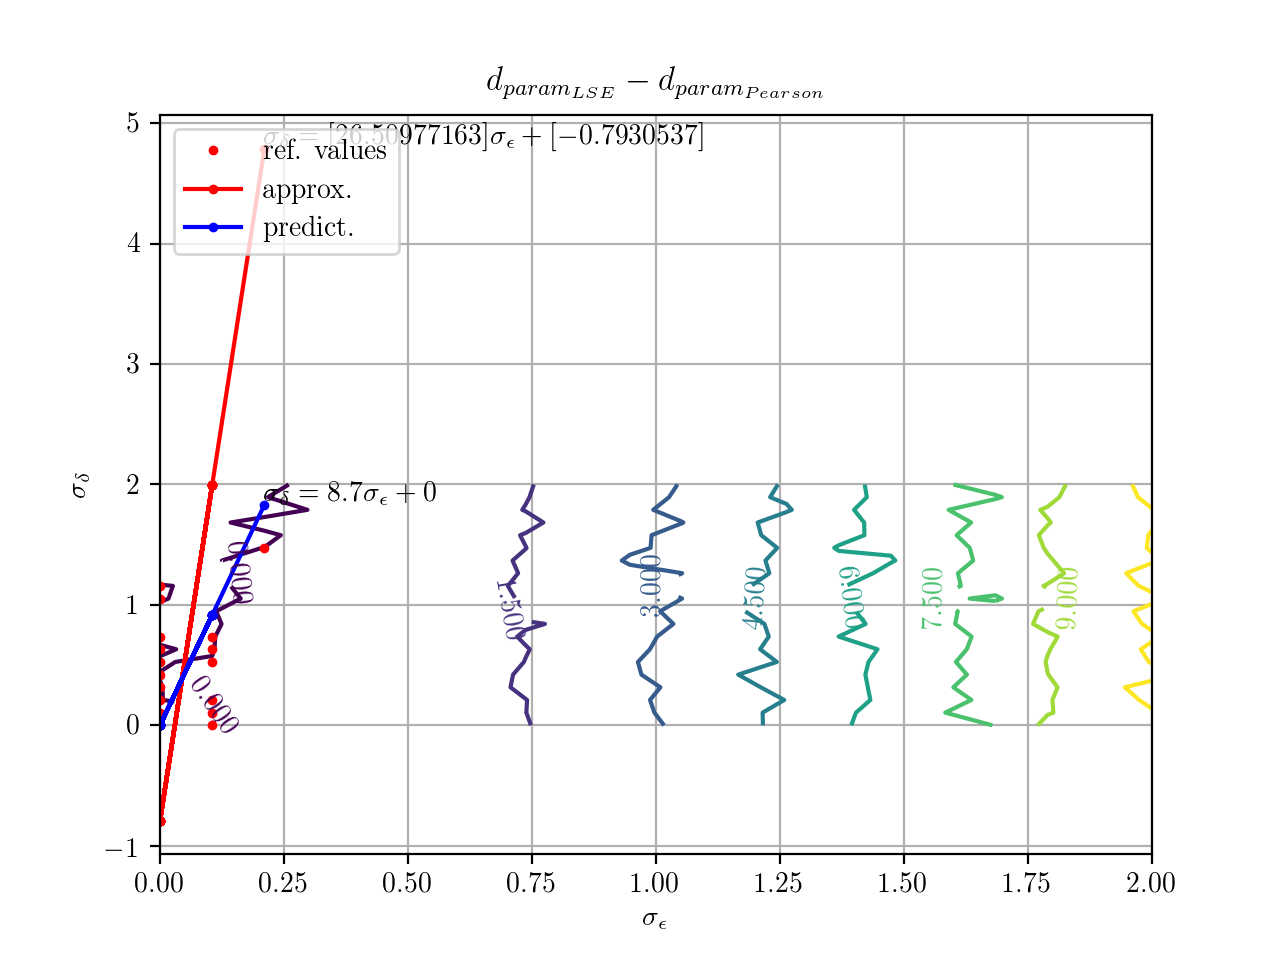
\includegraphics[width=.8\linewidth]{fig/beta-8_param-accs-diff-approx.png}
  \caption{$ \beta = 8 $}
\end{figure}

\end{document}
